% Preamble
\documentclass[../Relazione_circuiti]{subfiles}

% Packages

\graphicspath{{\subfix{../images/}}}

% Document
\begin{document}

\subsection{Analisi preliminare qualitativa}

  \begin{figure}[H]
    \centering

    \begin{subfigure}[b]{0.3\textwidth}
      \centering
      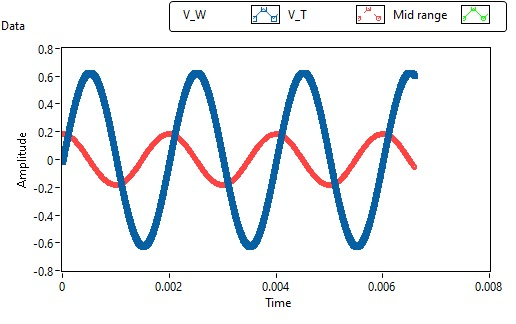
\includegraphics[width=\textwidth]{Cross_waveform_500.jpeg}

      \caption{Segnali a 500Hz}
      \label{fig:signal_500}

    \end{subfigure}
    \hfill
    \begin{subfigure}[b]{0.3\textwidth}
      \centering
      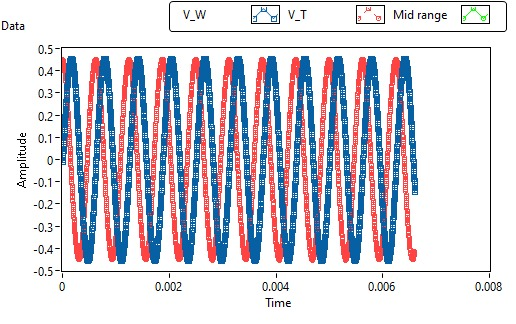
\includegraphics[width=\textwidth]{Cross_waveform_1600.jpeg}

      \caption{Segnali a 1600Hz}
      \label{fig:signal_1600}

    \end{subfigure}
    \hfill
    \begin{subfigure}[b]{0.3\textwidth}
      \centering
      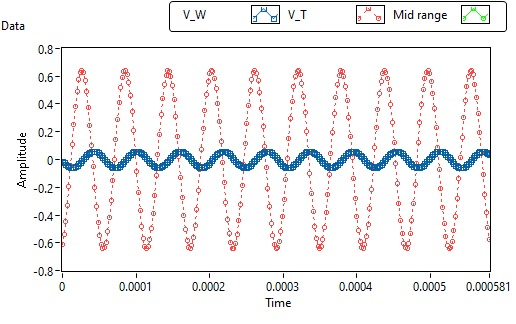
\includegraphics[width=\textwidth]{Cross_waveform_17000.jpeg}

      \caption{Segnali a 17kHz}
      \label{fig:signal_17k}

    \end{subfigure}

    \caption{Segnali osservati sui rami Woofer (blu) e Tweeter (rosso)
      a frequenza fissata. Le incertezze non sono visibili a causa della scala.}
    \label{fig:signal_waveforms}

  \end{figure}

  La Fig. \ref{fig:signal_waveforms} mostra la forma d'onda dei segnali osservati sui rami Woofer e Tweeter in risposta
  ad un segnale sinusoidale.
  La Fig. \ref{fig:signal_1600} mostra il comportamento nei pressi della frequenza di cross attesa, la Fig.
  \ref{fig:signal_500} a 1/3 e la Fig. \ref{fig:signal_17k} a circa 10 volte.

  Si osserva (Fig. \ref{fig:signal_1600}) che, coerentemente con quanto atteso, i segnali hanno ampiezza simile nei
  pressi di $f_{cross}$.
  A basse frequenze si osserva (Fig. \ref{fig:signal_500}) un'attenuazione del 60\% dell'ampiezza sul ramo Tweeter e
  nessuna alterazione sul Woofer, ad alte frequenze un'attenuazione sul Woofer dell'86\% e nessuna sul Tweeter (Fig.
  \ref{fig:signal_17k}).

\subsection{Analisi della frequenza misurata}

\subsection{Analisi dell'ampiezza}

  \begin{figure}[H]
    \centering

    \begin{subfigure}{=0.5\textwidth}

      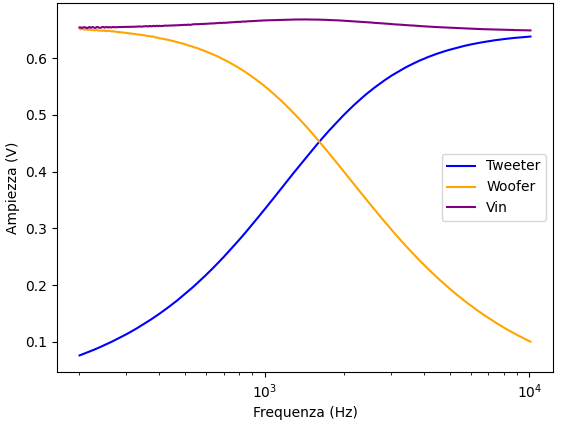
\includegraphics[width=\textwidth]{cross_dataonly.png}

      \caption{Andamenti sperimentali di Tweeter, Woofer e Vin (segnale in ingresso nel filtro,
        a valle della resistenza interna del generatore). Tensioni riferite al ground}
      \label{fig: amplitude_dataonly}

    \end{subfigure}

    \begin{subfigure}{=0.5\textwidth}

      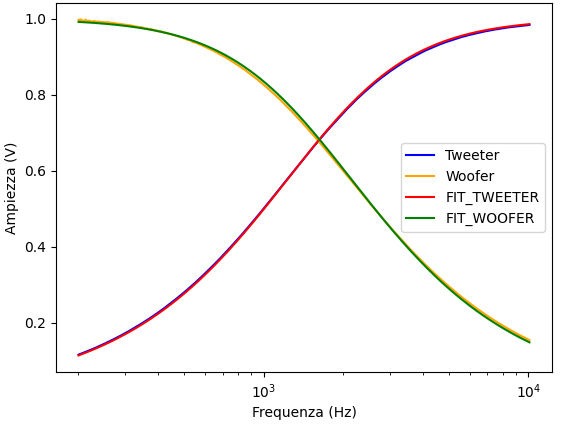
\includegraphics[width=\textwidth]{cross_gain_amplitude.png}

      \caption
      {Andamenti sperimentali e fit dei guadagni in tensione. Si noti la discrepanza tra la frequenza di cross e il
      massimo del Vin}
      \label{fig:cross_gain}
    \end{subfigure}

    \caption{Ampiezza misurata in funzione della frequenza (asse della frequenza in scala logaritmica)
      . A causa della scala le incertezze sulle singole misure non sono visibili. L'andamento è rappresentato da una
      linea continua a causa dell'alta densità di punti.}
    \label{fig:cross_amplitude}

  \end{figure}

  La Fig. \ref{fig:cross_amplitude} mostra l'andamento di ampiezza dei segnali filtrati in funzione della frequenza.

  La relazione funzionale Ampiezza massima-Frequenza (misurata ai capi della resistenza di carico dei rami) dipende
  dalla tensione in ingresso sul filtro $V_{in}$.
  Tuttavia, a causa della presenza della resistenza interna nel generatore e come visibile in Fig.
  \ref{fig: amplitude_dataonly}, la $V_{in}$
  dipende dalla frequenza ed assumerla costante potrebbe introdurre errori.
  Pertanto abbiamo calcolato i guadagni in tensione (Fig. \ref{fig:cross_gain}
  ) dividendo le ampiezze osservate per il valore di $V_{in}$
  osservato alla relativa frequenza, propagando le incertezze in quadratura.

  \begin{equation}
    G_{woofer} = \frac{1}{\sqrt{R^2+(\omega L)^2}}
  \end{equation}

  \begin{equation}
    G_{tweeter} = \frac{1}{\sqrt{R^2+(\frac{1}{\omega C})^2}}
  \end{equation}

%dove $V_{in}$ rappresenta la tensione in ingresso. %(assunta costante) pari a 0.65, osservata nel ramo Woofer nel
%    limite di basse frequenze e nel ramo Tweeter nel limite di alte frequenze.

%Le funzioni guadagno si ottengono semplicemente dividendo le eq date per vin (NOTA: da riscrivere, non voglio
%    duplicare le equazioni)

  E' stato effettuato un fit ai parametri L e C (R assunta costante). Da essi è stata poi ricavata la frequenza di
  crossover secondo l'Eq. \eqref{eq:f_cross}.

  \begin{table}
    \centering

    \begin{tabular}{c | c }

%Heading
      Grandezza & Valore                 \\

      L         & $(10.13 \pm 0.01)$ mH  \\
      C         & $(953.39 \pm 0.05)$ nF

    \end{tabular}

    \caption{Risultati del fit alle funzioni guadagno in tensione}
    \label{tab:fit_amplitude}

  \end{table}

  La Tab. \ref{tab:fit_amplitude} mostra i risultati del fit.
  Si osserva che la frequenza ottenuta non risulta compatibile con il valore teorico stimato \theoryF.
  Tuttavia, l'andamento della curva $V_{in}$ ci fornisce un metodo ulteriore per determinare la frequenza di cross.
  Infatti, a tale frequenza, si dimostra che l'impedenza totale del filtro è massima.
  Usando la legge di Ohm simbolica, ne segue che la tensione ai capi del filtro deve essere massima.
  Cercando il massimo della curva sperimentale, otteniamo il valore $(1434 \pm 8) \;$ Hz.
  L'incertezza è stata determinata considerando metà del passo di scansione utilizzato nei pressi di quella frequenza
  (come descritto in sezione 2, non è costante).

\subsection{Analisi della fase}

\end{document}